\begin{chapter}{Tools}

    An important process in the software development is the choice of the right
    tools, in order to achieve simplicity and efficiency for both development
    process and the project itself.
    In this chapter will be described the main tools used during the development
    of Restlessness and its deployment to make its use available to everyone.

    \section{JavaScript}
    JavaScript is a lightweight interpreted programming language. Interpreted means
    that the code is read top to bottom, and the result of the running code is
    immediately returned. Interpreted programming languages are opposed to compiled
    one, where the code is transformed into a binary format that can be directly
    executed \cite{what_is_js}.
    Although JavaScript was born as a language limited to client side programming,
    exploiting an engine directly incorporated into the Web browser, with the
    introduction of Node.js has become possible to use this language also for backend
    programming, and in general in contexts outside of the browser.
    Node.js is a JavaScript runtime based on the V8 engine, on which the popular
    Chrome browser is based \cite{node_org}.
    A key characteristic and one of the main strength of JavaScript with respect
    to other programming languages is its asynchronous nature, that allows having
    non-blocking I/O. As a consequence of this the code runs on a single thread,
    based on a LIFO queue (Last In, First Out) continuously checked by the so called
    Event Loop.
    As shown on \ref{fig:event_loop}, operation regarding File System, Network or
    Database access are executed separately and only once completed are inserted
    again into the queue, to handle their result, meanwhile other queued code
    is executed by the only present thread.

    \begin{figure}
        \centering
        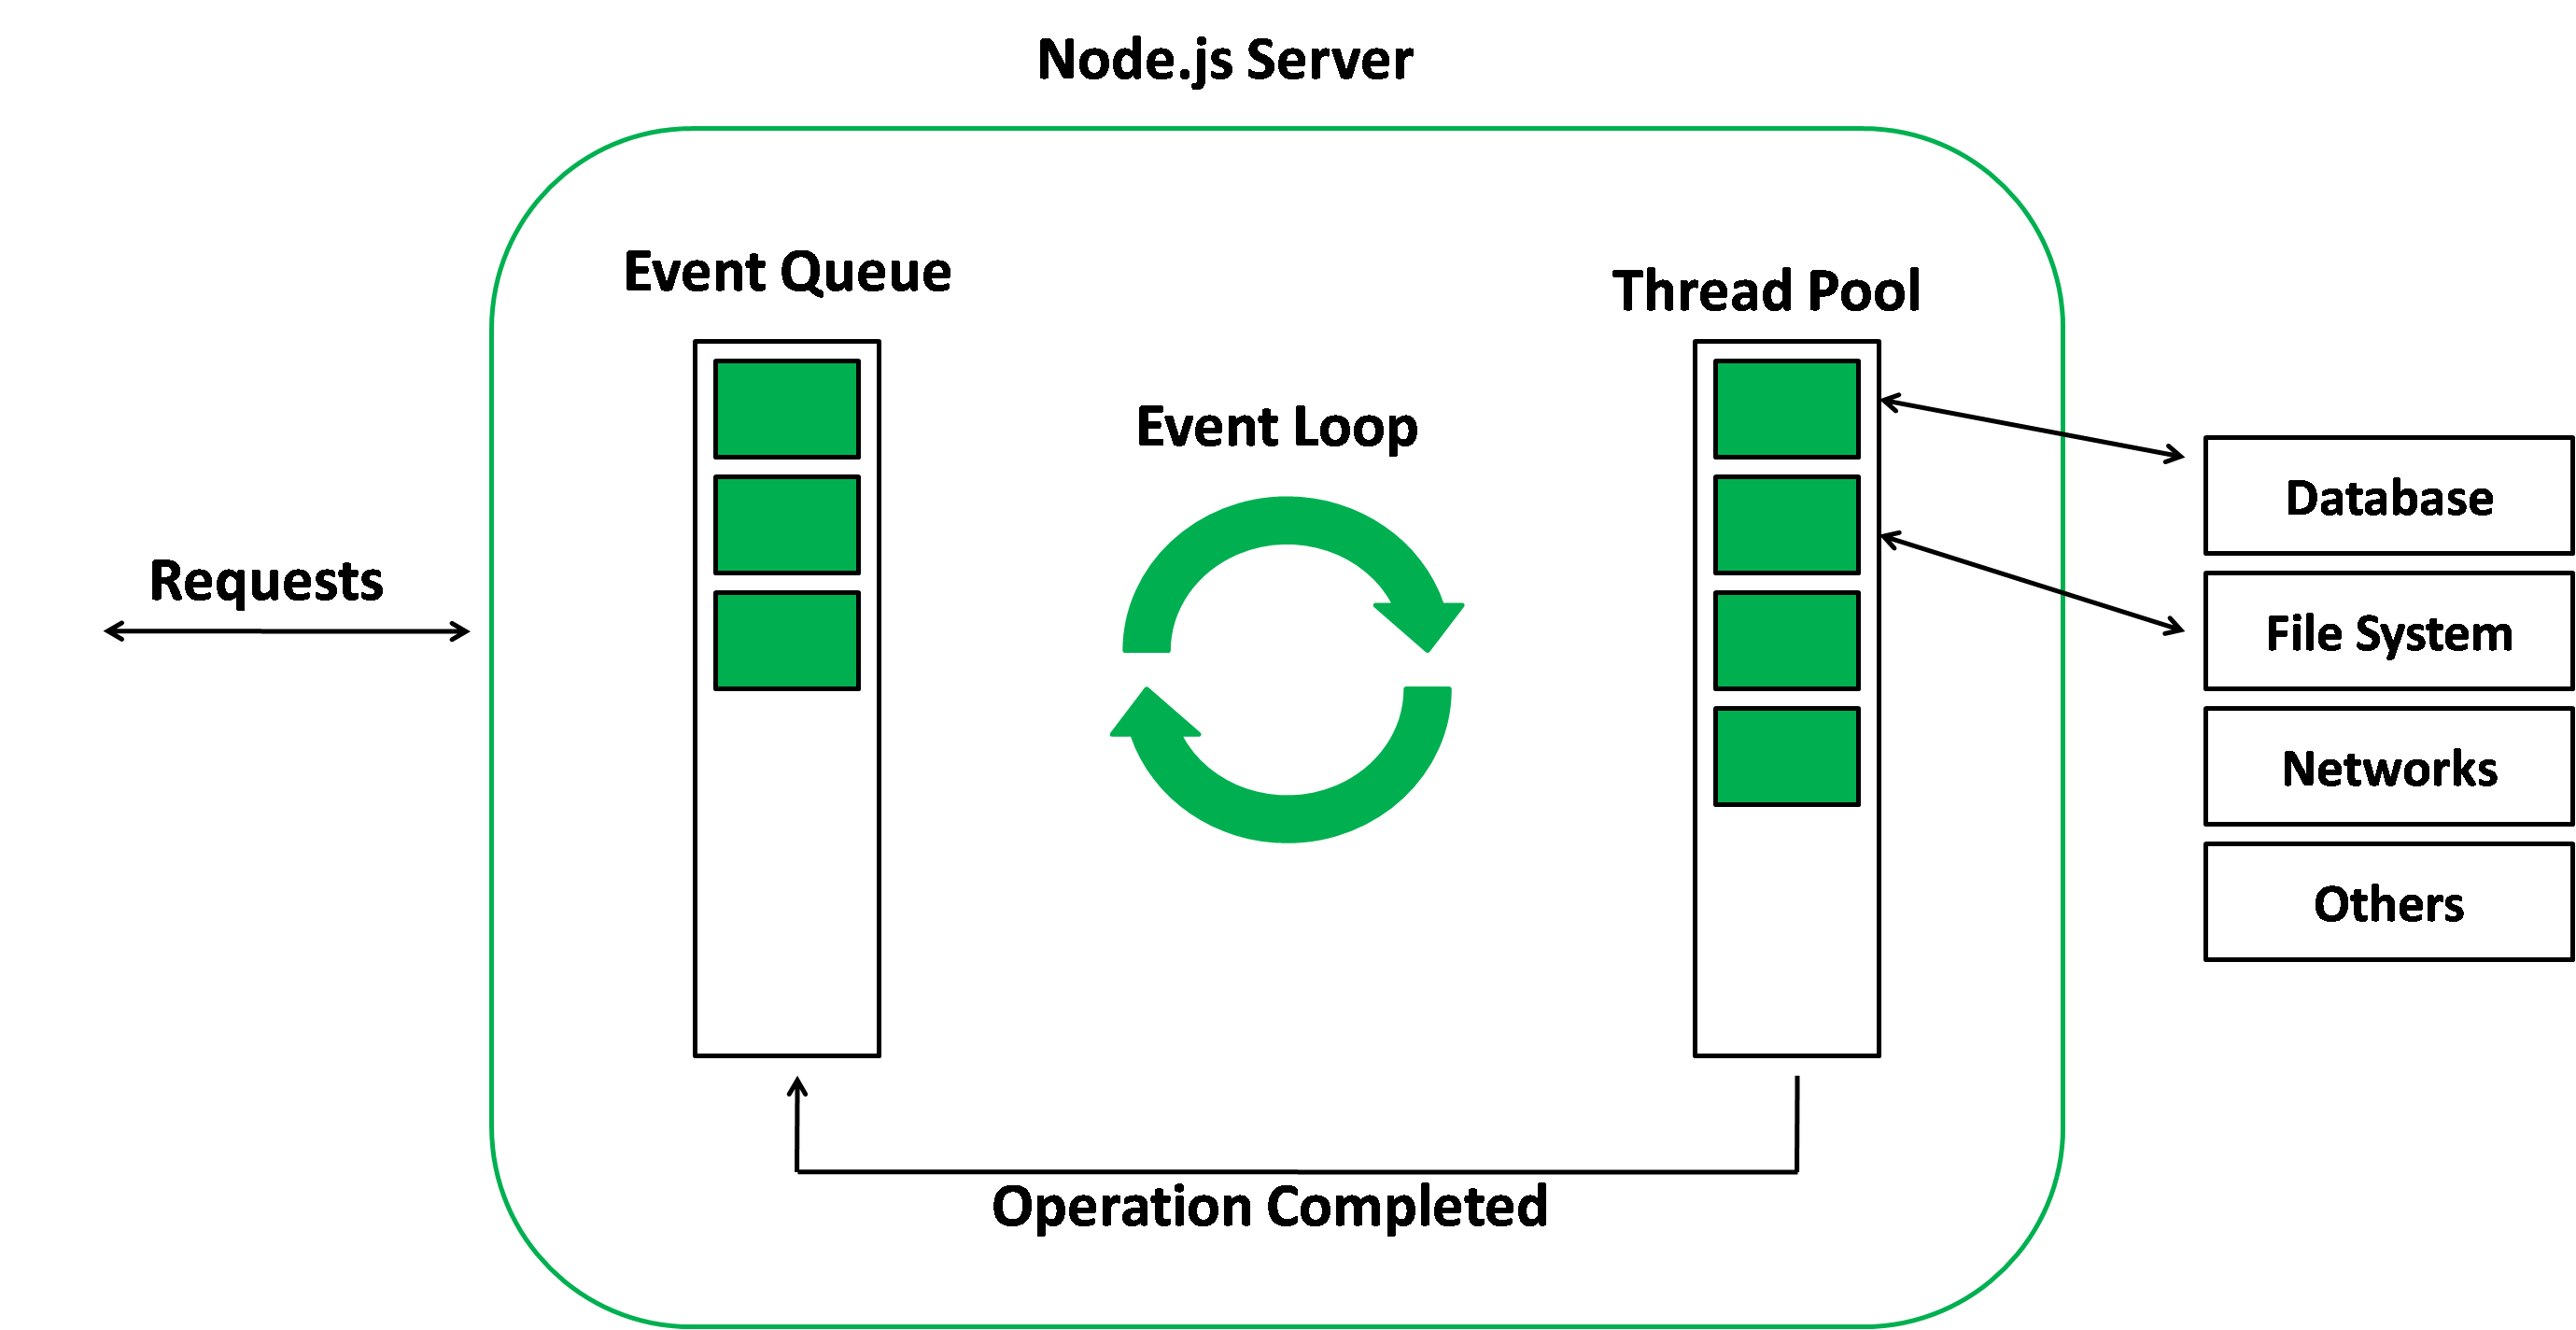
\includegraphics[width=\linewidth]{source/images/nodejs_event_loop.png}
        \caption{The Event Loop \cite{node_event_loop_2}}
        \label{fig:event_loop}
    \end{figure}

    Being single threaded is a useful limitation as it's not possible to incur
    into concurrency issues.
    This peculiarities make JavaScript well suited for the so called real-time
    applications (RTAs), that is applications that have to process a high volume
    of short messages requiring low latency, and so they require a highly scalable
    solution. Conversely due to its single threaded nature, JavaScript is not
    recommended for CPU-heavy jobs, as the Event Loop would be stuck on a single
    operation \cite{node_event_loop}\cite{node_on_backend}.

    Another advantage of JavaScript, especially after the release of Node.js, is
    the possibility to use the language for both frontend and backend in the context
    of Web development, creating a seamless experience for developers.

    JavaScript is a dynamically typed language, which means that it's not necessary
    to explicitly mention the type of data a variable holds, as that type can change
    dynamically as change the content of the variable (\ref{lst:dynam_type}).

    \begin{code}[caption=Dynamically typed variables, label={lst:dynam_type}]
let a = "Hello World!"
a = 42
    \end{code}

    This feature of the language gives a lot of flexibility to developers, however
    as the project complexity grows it can quickly become a downside.
    For this reason, in 2012 Microsoft released an open source language called
    Typescript, a superset of JavaScript that enable static type checking.
    Being a superset, any JavaScript code is also valid Typescript code, enabling
    a gradual integration for already existing code bases.
    The Typescript compiler is specifically a transpiler, or a compiler that take
    source code as input and produces other source code as output, in this case
    JavaScript code. The compiler will point the errors it encounters, but it does
    not prevent the code to be run, hence it behaves like a spellchecker for the code.
    Typescript can also infer variables type from their usage, reducing the effort
    needed to enable static type checking from the developer
    \cite{typescript_lang}\cite{typescript}.
    Keeping in mind the described strengths of the JavaScript environment, has been
    decided to use it as the main language for the development of the Restlessness
    framework.

    \bigskip
    \begin{code}[caption=Static type checking on Typescript, label={ts_static}]
interface Student {
  name: string
  graduationYear: number
}

const aStudent: Student = {
  name: 'Arthur Dent',
  graduationYear: 2020
}

aStudent.graduationYear = '2020'    // Invalid
aStudent.graduationYear = 2021      // Valid
    \end{code}

    \section{Npm}
    The strengths of the JavaScript ecosystem are further increased by the presence
    of Npm, shorthand for Node Package Manager, which is the official package Manager
    for Node.js. Npm rely on the commonjs modules specification \cite{common_js},
    which defines a convention for the JavaScript module ecosystem.
    The main components of Npm are:
    \begin{itemize}
        \item Npm registry: modules can be published to it or installed from it.
            The official and main registry is available at the address
            \url{https://npmjs.org}
        \item \textit{npm} CLI: the command line tool from which is possible to interact
            with the registry, with operations like publishing or installing packages.
        \item \textit{package.json}: a configuration file, in the Json format
            \cite{json_iso}, that must be present for both modules that are published
            into the registry and modules that use other modules from the registry
            as dependencies. It contains projects information, such as name and
            version, and a list of other modules, on which the project depends on.
        \item \textit{node\_modules}: an automatically created folder that contains
            all the projects dependencies. At runtime Node.js looks for modules
            in this folder.
    \end{itemize}

    Listing \ref{lst:add_module} shows the \textit{package.json} of a simple module,
    while \ref{lst:add_fn} shows the definition of a function, on that module,
    exported using the CommonJs specification. To publish the package on the Npm
    registry is possible to invoke the \textit{publish} command on the \textit{npm}
    CLI. With the \textit{install} command that same package is installed as
    dependency under the \textit{node\_modules} folder, and can be used as shown
    on listing \ref{lst:add_require}

    \bigskip
    \begin{code}[caption=A simple \textit{package.json},
        label={lst:add_module}, language=json]
{
    "name": "add_module",
    "version": "1.0.0",
    "description": "Simple module example",
    "main": "index.js",
    "author": "Arthur Dent",
    "license": "ISC"
}
    \end{code}

    \bigskip
    \begin{code}[caption=CommonJs module definition, label={lst:add_fn}]
// index.js
function add(n1, n2) {
  return n1 + n2
}

module.exports = add
    \end{code}

    \bigskip
    \begin{code}[caption=CommonJs module usage, label={lst:add_require}]
const add = require('./add.js')
    \end{code}

    The Npm ecosystem has been used extensively during the development of Restlessness,
    for its dependencies and for making it available on the registry.
    Furthermore, the developed framework uses a feature of Npm called Scoped Packages
    \cite{npm_scoped_packages}, which allows to group related packages together
    under a common scope, acting as a namespace. Restlessness packages are available
    under the \textit{@restlessness/} scope.

    \section{Github}
    \subsection{Git}
    Git is an Open Source Distributed Version Control System, in particular:
    \begin{itemize}
        \item Control System: Git is a content tracker, it can be used to store
            content, which generally is code.
        \item Version: the tracked content is subject to continuous change, often
            this changes are added in parallel. Git helps handling this by maintaining
            a history of all changes.
        \item Distributed: Git is based on remote and local repositories, the first
            one stored in a server, while the latter is stored in the developer
            computer, and both contains the full history information.
    \end{itemize}

    Git is useful to track code changes in all cases, but it's absolutely necessary
    to avoid conflicts when multiple developers work in parallel on a single codebase.
    The main concepts introduced by Git are:
    \begin{itemize}
        \item Commit: the main unit representing content modification.
        \item Branches: allows working simultaneously at the codebase, making
            different modifications.
        \item Push/Pull: operations that allow synchronization between the remote
            repository and the local one.
        \item Merge: operation that integrate the modification made on a branch
            into another branch.
        \item Tag: a string identifier assigned to a specific commit, useful to
            reference a particular version of the project (e.g. a simple tag is
            \textit{v1.0.2}).
    \end{itemize}

    \begin{figure}
        \centering
        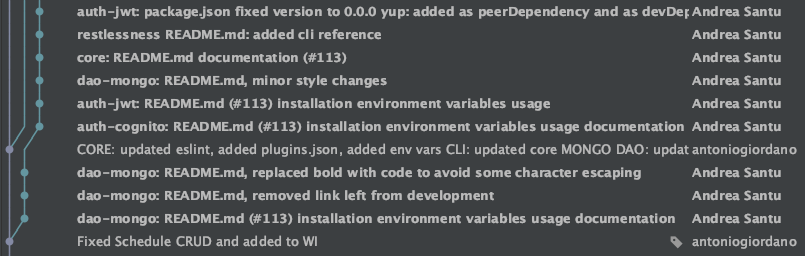
\includegraphics[width=\linewidth]{source/images/rln-git-history.png}
        \caption{Section of Restlessness history}
    \end{figure}

    With these concepts it is possible to work on each feature independently from
    others, integrating it only when it reaches an appropriate stability level.
    The strategy adopted with the developed framework has been to create branches
    with the \textit{feature/} prefix for new functionalities or improvement of
    existing ones, and the \textit{fix/} prefix for correction of bugs, followed
    by the name of the specific feature of fix.

    \subsection{Github features}
    Github is a web based platform providing all functionalities offered by the Git
    system plus additional DevOps features, with the main ones used during the
    development of Restlessness being: Issues, Pull Requests and Projects.

    \subsubsection{Issues}
    Issues are Github feature that helps to keep track of tasks, bugs, enhancements
    or any kind of modification to the project. They are characterized by a title,
    that gives an immediate feedback about what is the reason of the Issue, and an
    optional description, with more specific and technical information, as shown
    on figure \ref{fig:rln_issue}. Each Issue can be assigned to one or more
    collaborators, responsible for having it solved. This tracking system is focused
    on collaboration, as it is possible to comment and discuss about the Issue with
    other collaborators, also referencing other resources, which can be other Issues
    or code sections.
    As the project grows so does the number of Issues, and so become important to
    keep them organized. This is made possible by using Labels and Milestones.
    Both allow to group Issues according to a common characteristic, but with a
    different granularity \cite{github_issues}.
    The first one allows a more specific grouping, with the main ones defined for
    Restlessness being:
    \begin{itemize}
        \item \textit{enhancement}: A new feature, or a request for a new feature.
        \item \textit{bug}: A problem in the project functionalities.
        \item \textit{documentation}: Improvements or additions to documentation.
        \item \textit{tests}: Testing related Issues
        \item \textit{good first issue}: Being the framework Open Source, also
            external people can contribute to it, this Label marks simple and easy
            Issues that can be managed also by newcomers.
        \item Packages specific Issues: Restlessness adopt a monorepo  strategy
            \cite{monorepo}, having all provided packages under the same repository,
            so it has been defined a Label for each package, such as: \textit{CORE},
            \textit{CLI}, \textit{AUTH-cognito} and \textit{DAO-mongo}.
    \end{itemize}
    The latter instead group together Issues linked together from a temporal point
    of view, typically a version release or a planned Sprint if following the agile
    methodology \cite{agile}. With the Restlessness framework has been opted for
    the first option.


    \begin{figure}
        \centering
        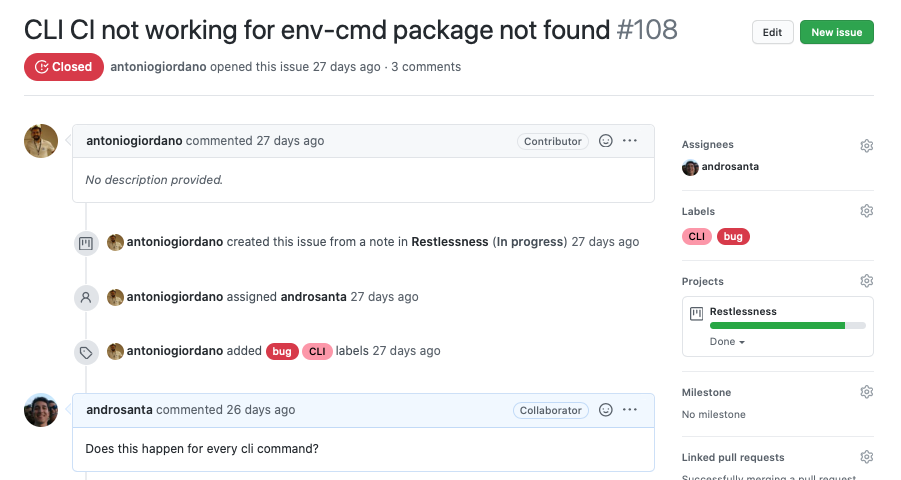
\includegraphics[width=\linewidth]{source/images/github-rln-issue.png}
        \caption{An Issue on the Restlessness project}
        \label{fig:rln_issue}
    \end{figure}

    \begin{figure}
        \centering
        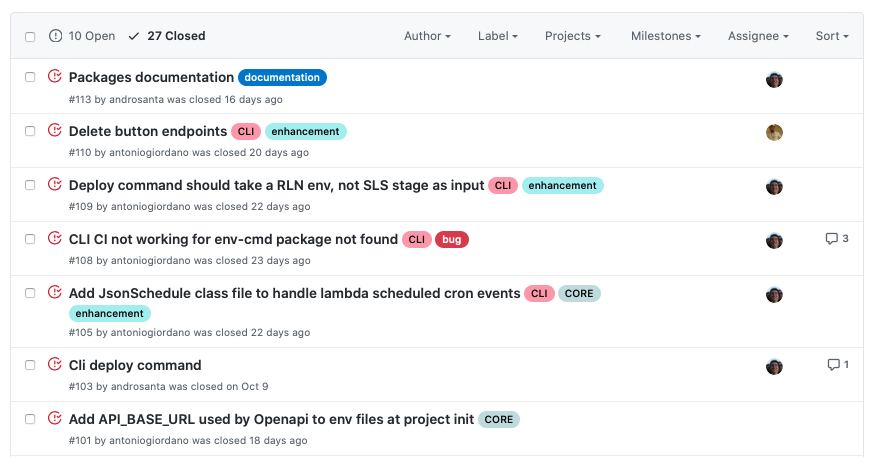
\includegraphics[width=\linewidth]{source/images/github-rln-issues-list.png}
        \caption{List of closed Restlessness Issues}
        \label{fig:rln_issues_list}
    \end{figure}

    \subsubsection{Pull Requests}
    An important process when multiple developers collaborate on a single project
    are code reviews, as having project's modification verified by more than one
    person reduces the risk for finding bugs, typos and critical problems later.
    Pull Requests are a feature of Github that enable this process, with it a
    collaborator proposes its changes while another one accept or reject the request.
    It is possible to discuss on the specific request, referencing other resources,
    commenting on code or requesting modification on the proposed changes, as it
    happens for Issues.
    When a Pull Request is created the author chose a target branch on which to
    integrate its proposed changes, and once the request is accepted those changes
    are merged into the target branch, and the Pull Request is considered closed,
    as shown on figure \ref{fig:rln_pull_request}.

    \begin{figure}
        \centering
        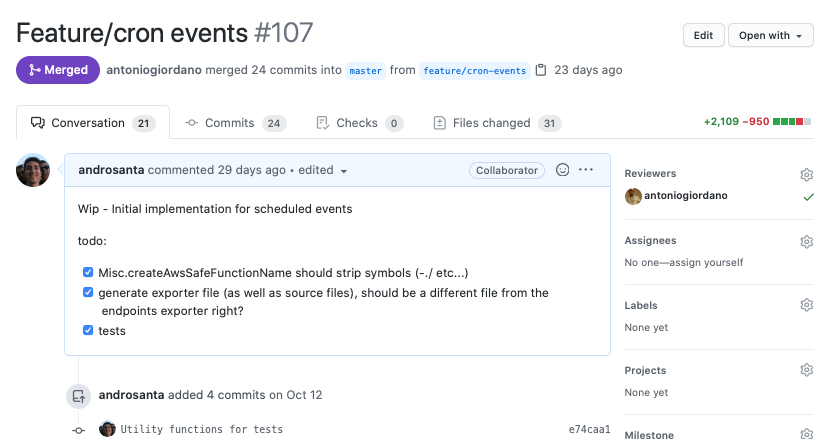
\includegraphics[width=\linewidth]{source/images/rln-pull-request.png}
        \caption{An approved Pull Request on the Restlessness project}
        \label{fig:rln_pull_request}
    \end{figure}

    \subsubsection{Projects}
    Projects is a recently added Github feature with the purpose of further improve
    organizing and distributing tasks and work. From the Projects page is possible
    to define custom columns in which assign different tasks, which can be Issues,
    Pull Requests or simple Notes. As shown in figure \ref{fig:rln_project_board},
    for Restlessness has been defined tree columns: \textit{To do},
    \textit{In Progress} and \textit{Done}. This way it is immediately visible which
    tasks need to be done, are under development or are already completed.

    \begin{figure}
        \centering
        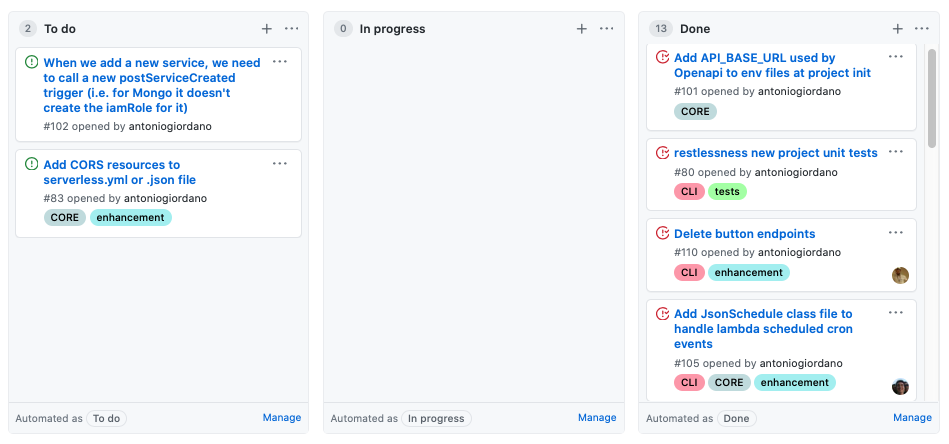
\includegraphics[width=\linewidth]{source/images/rln-github-project-board.png}
        \caption{Github Projects board on Restlessness}
        \label{fig:rln_project_board}
    \end{figure}

    \bigskip
    \bigskip
    \noindent
    Being the developed framework Open Source, it is available for consultation,
    modification and improvement on Github, as well as this document, on the
    following addresses:
    \begin{itemize}
        \item Restlessness: \url{https://www.github.com/getapper/restlessness}
        \item Thesis: \url{https://www.github.com/androsanta/Thesis}
    \end{itemize}

    \section{CircleCi}

    \subsection{CI/CD}
    Continuous Integration is a practice that encourages developers to integrate
    their code changes early and often, into the main and stable version of the
    project, which for a git based project is the \textit{master} branch.
    Each code integration triggers an automated build and test, that if failed can
    be repaired quickly.
    The main advantage of using this approach is the early bug detection, which
    as consequence will result in an overall reduced bug count and reduced
    maintenance. Moreover once set, the CI process does not add any overhead to
    the development as it is completely automated.
    The CI approach is oftentimes related to another approach, which is the
    Continuous Delivery, defined as
    \enquote*{%
        Continuous Delivery (CD) is a software engineering approach in which teams
        keep producing valuable software in short cycles and ensure that the
        software can be reliably released at any time.%
    } \cite{continuous_delivery}

    \subsection{The platform}
    CircleCi is an online platform that provides services for implementing
    Continuous Integration and Continuous Delivery (CI/CD) on software projects.
    It can be configured to access the source code repository on Github, and after
    that each commit can trigger an automated build, test and deploy task.
    Those automated tasks are performed inside a clean container or Virtual Machine,
    ensuring a reproducible environment.

    \begin{figure}
        \centering
        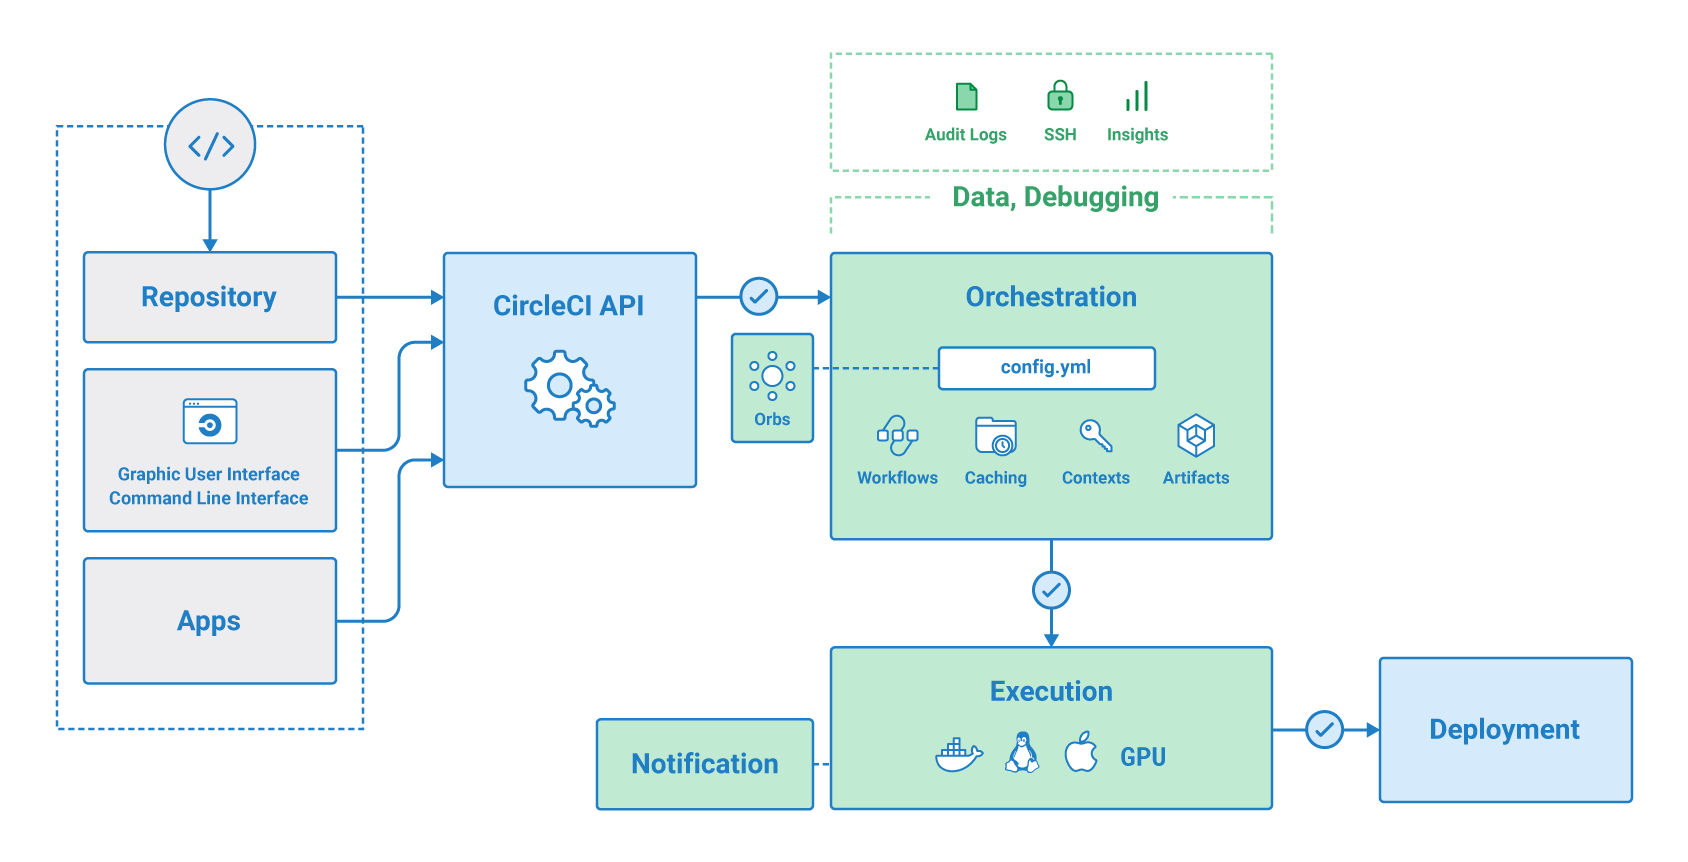
\includegraphics[width=\linewidth]{source/images/circle-ci.png}
        \caption{CircleCi flow \cite{circle_ci_official}}
        \label{fig:circle_ci_structure}
    \end{figure}

    The main concepts introduced by the platform are:
    \begin{itemize}
        \item Configuration: All processes are orchestrated through a single file
            called \textit{config.yml}, in the \href{https://yaml.org/}{Yaml} format,
            and placed under a folder called \textit{.circleci} at the root of the
            project.
        \item Orbs: Reusable snippets of code that help automate repeated processes
        \item Jobs: Building blocks of the configuration file, they are a collection
            of steps, which run commands or scripts as specified. Each Job is run
            in a unique executor.
        \item Executor: The container or Virtual Machine where running each Job.
            It is possible to chose between \href{https://www.docker.com/}{Docker}
            containers, Virtual Machines running Linux, Windows or MacOS.
        \item Steps: Actions that need to be taken to complete a Job. It can be
            any kind of executable command.
        \item Workflows: They define a list of Jobs and their run order, and
            concurrency.
    \end{itemize}

    For the Restlessness development has been chosen the popular containerization
    solution \href{https://www.docker.com/}{Docker}, in particular a Node.js based
    container, as shown on listing \ref{lst:ci_executor}:

    \bigskip
    \begin{code}[caption=Reusable executor definition, label={lst:ci_executor},
        language=yaml]
executors:
  node12:
    docker:
      - image: circleci/node:12.9.1
    \end{code}
    As previously said the framework adopt a monorepo structure, so has been necessary
    to define multiple Workflows, one for each package. Each Workflow defines two
    parallel Jobs, for testing and publishing on the Npm registry.
    Figure \ref{fig:ci_workflow_diagram} show the described structure for two Restlessness
    packages, and it is possible to notice that each Job run in its own container,
    in parallel and independently from the others

    \begin{figure}
        \centering
        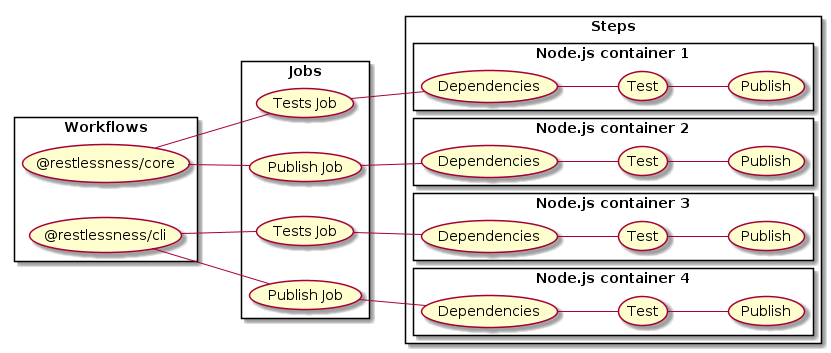
\includegraphics[width=\linewidth]{source/diagrams/ci_workflow.png}
        \caption{CircleCi workflows for Restlessness}
        \label{fig:ci_workflow_diagram}
    \end{figure}

    To perform the Steps shown on \ref{fig:ci_workflow_diagram} has been defined
    reusable commands, with the main one being:
    \begin{itemize}
        \item \textit{install\_packages}: Install dependencies as specified by the
            \textit{package.json}.
        \item \textit{deps\_and\_tests}: Install dependencies and run tests as
            specified by the \textit{package.json}.
        \item \textit{npm\_publish}: Publish the package on the Npm registry.
    \end{itemize}

    According to the Continuous Delivery approach the publish operation is triggered
    manually by performing a git tag on a specific repository commit, following the
    format: package name, followed by \textit{/v} and the semantic version of the
    package (e.g. \textit{@restlessness/core/v1.0.2}). A custom script takes care
    of extractive the version information and set it on the correct \textit{package.json},
    where is read from the npm publish command.

    Although CircleCi offers its own website from which is possible to check Workflow
    execution, errors and details of every operation, it offers also a Github plugin,
    that is able to show Workflows result directly on commits or Pull Requests, as
    shown on \ref{fig:ci_github_integration}. The integration between the two
    services has simplified the development workflow of Restlessness, and adds to
    the already described advantages of adopting a CI/CD approach.



    \begin{figure}
        \centering
        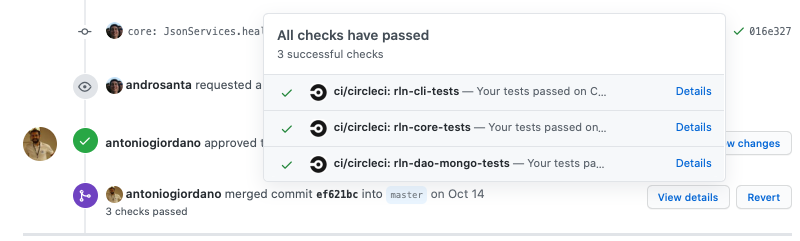
\includegraphics[width=\linewidth]{source/images/ci-github-integration.png}
        \caption{CircleCi Workflows seen from Github}
        \label{fig:ci_github_integration}
    \end{figure}

    \section{AWS}
    Amazon Web Services is a cloud platform offered by \textit{Amazon.com, Inc}
    which, between its various services, also provides serverless computing options.
    Although one of the purpose of using the Serverless Framework is to abstract
    the underlying infrastructure details of the platform, those details are needed
    to develop a framework such as Restlessness, that has to interact with the
    platform at a lower level to provide its functionalities.

    Here is a list of the main services used by Serverless and Restlessness on
    behalf of the user and also used during Restlessness development:
    \begin{itemize}
        \item Lambda: The compute service providing the serverless functionalities.
            A Lambda function contains the code written by the developer.
        \item API Gateway: A service that creates a connection point between
            external requests and other internal services, such as a Lambda function.
        \item S3: Acronym for Simple Storage Service, provides object storage.
            Resources are organized in container called Buckets.
        \item CloudFormation: A service that allow to model infrastructure as code.
            Each CloudFormation configuration corresponds to a resource called
            CloudFormation Stack, containing the description of other resources,
            such as AWS Lambda functions, API Gateway, and how such resources may
            interact.
        \item CloudWatch: A services for monitoring and observability.
        \item IAM:Acronym for Identity and Access Management, enables the management
            of AWS resources access.
    \end{itemize}

    \subsubsection{Resource creation during deploy}
    During the deployment of a Serverless service the user code and its dependencies
    are packaged into a zip artifact, then begin the remote resource creation of
    a CloudFormation Stack and an S3 Bucket. One that resources initialization has
    been completed, the CloudFormation configuration and the zip artifact are uploaded
    and saved into the S3 Bucket and that operation is followed by the creation of
    all resources defined on the CloudFormation Stack. Those operations are shown
    on figure \ref{fig:sls_deploy_on_aws}

    \begin{figure}
        \centering
        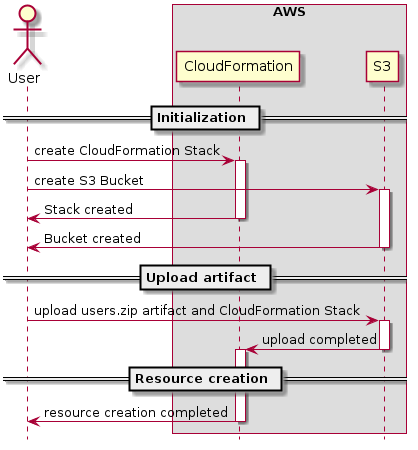
\includegraphics[width=8cm]{source/diagrams/sls_deploy_on_aws.png}
        \caption{Resources creation on Serverless deploy for a \textit{User} service}
        \label{fig:sls_deploy_on_aws}
    \end{figure}

    \subsubsection{Lambda function invocation through an API Gateway}
    \label{subsec:lambda_invocation}

    Figure \ref{fig:simple_lambda} shows the simplest possible case of execution
    flow of an http request, handled by an API Gateway, and forwarded to the Lambda
    function mapped to the user specified endpoint path.

    \begin{figure}
        \centering
        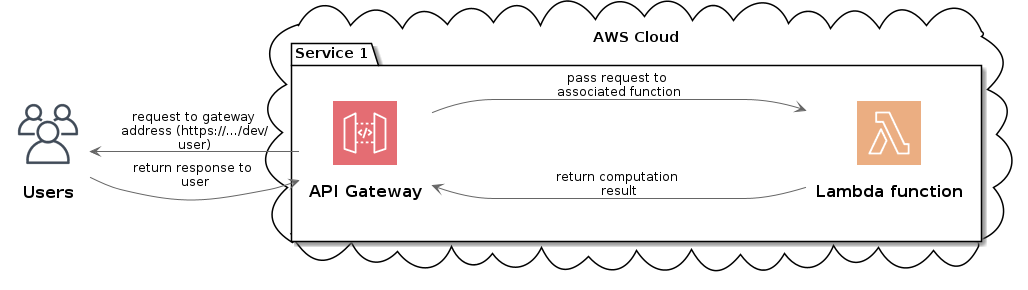
\includegraphics[width=\linewidth]{source/diagrams/lambda_invocation.png}
        \caption{Simple Lambda function execution through an API Gateway}
        \label{fig:simple_lambda}
    \end{figure}

    A more complex case is given when implementing user Authentication and hence
    restricting Lambda execution. The Authentication process is made simple by
    delegating the operation of granting or denying Authentication to a Lambda
    function, called Lambda Authorizer \cite{aws_api_gateway_doc}, as shown on
    figure \ref{fig:lambda_with_auth}. There can be two types of Lambda Authorizers:
    \begin{itemize}
        \item TOKEN: the Lambda receives the caller's identity in a bearer token.
        \item REQUEST: the Lambda receives the caller's identity in a combination
            of headers and query string parameters.
    \end{itemize}

    \begin{figure}
        \centering
        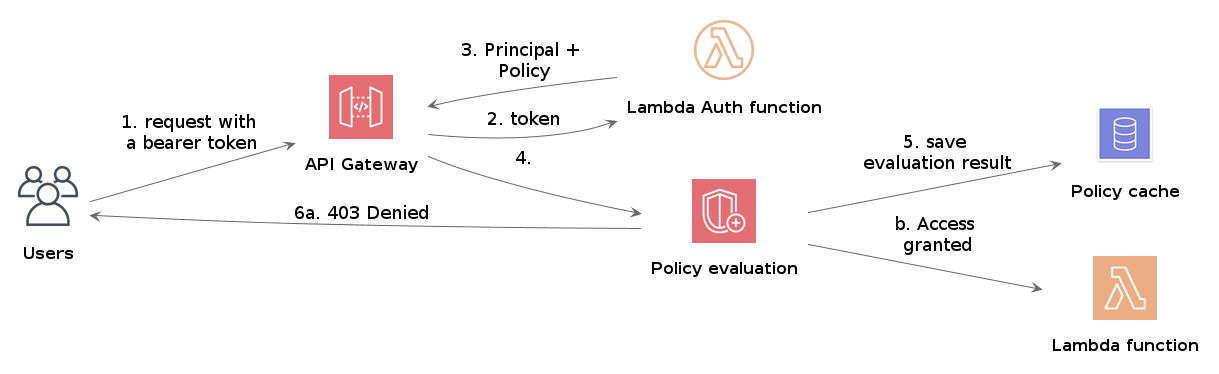
\includegraphics[width=\linewidth]{source/diagrams/lambda_authorizer.png}
        \caption{Lambda Authorizer function, based on TOKEN identity}
        \label{fig:lambda_with_auth}
    \end{figure}

    The API Gateway forward the request to the specified Lambda Authorizer, that
    checks the caller's identity and generate an Authentication Policy, which is
    an object that states which resources the user is authorized to access.
    The Policy is then cached to improve performance on subsequent requests, and
    if it the access request is granted, the flow proceed as in the previously
    described case.

    Serverless abstract this structure by allowing to specify a function as
    Authorizer of another function, as shown on listing \ref{lst:sls_auth}, where
    the \textit{getUsers} function is executed only if the function \textit{auth}
    grants access.

    \bigskip
    \begin{code}[caption=Authorizer definition on Serverless, label={lst:sls_auth},
        language=yaml]
functions:
  auth:
    handler: auth.customAuth  # auth.js
  getUsers:
    handler: users.getUsers   # users.js
    events:
      - http:
        path: hello
        method: get
        authorizer: auth
    \end{code}

    \section{React}
    An important part of the Restlessness framework is its Graphical User Interface,
    which is the main interaction point for the user. The Frontend development,
    specifically toward Web Interfaces, can count on the presence of several
    libraries and frameworks based on the JavaScript language. For the development
    of Restlessness has been chosed the popular library React, due to its simplicity,
    and effectiveness.

    React is an Open Source JavaScript library that implements the concept of
    virtual DOM (Document Object Model) \cite{dom_standard}. The browser creates
    a DOM object at page loading, and then each Html object inside the DOM can be
    manipulated using JavaScript functions, giving the user an immediate feedback.
    React instead adopt a different approach by creating a virtual DOM alongside
    the real one. The virtual DOM is not directly synched with the real one, so
    it can be modified much faster, not having to reflect those modification on
    the screen. After those virtual DOM updates are created using the React api,
    the new istance of the virtual DOM is compared to the previous one, allowing
    to reflect the update on the real DOM only for the elements that actually
    change. The library allow to create a structure based on reusable component,
    obtaining a scalable structure, and is particularly suited for SPA (Single
    Page Applications) \cite{react_js}.
    The library also introduced a new syntax, named JSX (JavaScript XML), and
    listing \ref{lst:react_example} show the definition of a React component.

    \bigskip
    \begin{code}[caption= React component definition,label={lst:react_example}]
import React from 'react';

const Card = ({name}) => {
  return (
      <div>{name}</div>
  );
};
    \end{code}

\end{chapter}